% !TEX root = MusicFormatsMaintainanceGuide.tex

% -------------------------------------------------------------------------
\chapter{MusicFormats distributions}\label{MusicFormats distributions}
% -------------------------------------------------------------------------

The \mf\ \repo\ is hosted by \github\ and uses so-called \MainIt{actions} to build the library on \MacOS, \Ubuntu\ and \Windows. The resulting files are then uploaded to the \repo, where they are available to create the distributions for these three \OS s.


% -------------------------------------------------------------------------
\section{GitHub actions}
% -------------------------------------------------------------------------

These actions are defined in \code{.yml} files in \directoryName{.github/workflows}:
\begin{lstlisting}[language=Terminal]
jacquesmenu@macmini: ~/musicformats-git-dev/.github/workflows > ls -sal
total 32
0 drwxr-xr-x  6 jacquesmenu  staff   192 Feb 19 08:07 .
0 drwxr-xr-x@ 4 jacquesmenu  staff   128 May  5  2021 ..
8 -rw-r--r--@ 1 jacquesmenu  staff  1285 Feb 11 17:55 macos-check.yml
8 -rw-r--r--@ 1 jacquesmenu  staff  1343 Feb 11 17:55 ubuntu-check.yml
8 -rw-r--r--@ 1 jacquesmenu  staff  1396 Feb 11 17:55 windows-check.yml
\end{lstlisting}

For example, the \Ubuntu\ action in \file{ubuntu-check.yml} is:
\begin{lstlisting}[language=Terminal]
# This is a basic workflow to help you get started with Actions

name: Ubuntu

# Controls when the action will run.
on:
  # Triggers the workflow on push or pull request events but only for the master branch
  push:
    branches: [ master ]
  pull_request:
    branches: [ master ]

  # Allows you to run this workflow manually from the Actions tab
  workflow_dispatch:

# A workflow run is made up of one or more jobs that can run sequentially or in parallel
jobs:
  # This workflow contains a single job called "build"
  build:
    # The type of runner that the job will run on
    runs-on: ubuntu-latest

    # Steps represent a sequence of tasks that will be executed as part of the job
    steps:
      # Checks-out your repository under $GITHUB_WORKSPACE, so your job can access it
      - uses: actions/checkout@v2

      - name: Build MusicFormats for Ubuntu
        run: make -C build

      - name: Upload libraries and executables for Ubuntu
        uses: actions/upload-artifact@v2
        with:
          name: musicformats-ubuntu-distrib
          path: |
            MusicFormatsVersionNumber.txt
            build/bin
            build/lib/*.a
            build/lib/*.so
            documentation/IntroductionToMusicXML/IntroductionToMusicXML.pdf
            documentation/MusicFormatsCLIUserGuide/MusicFormatsCLIUserGuide.pdf
\end{lstlisting}

After a push to the \masterBranch, we get for example:\\
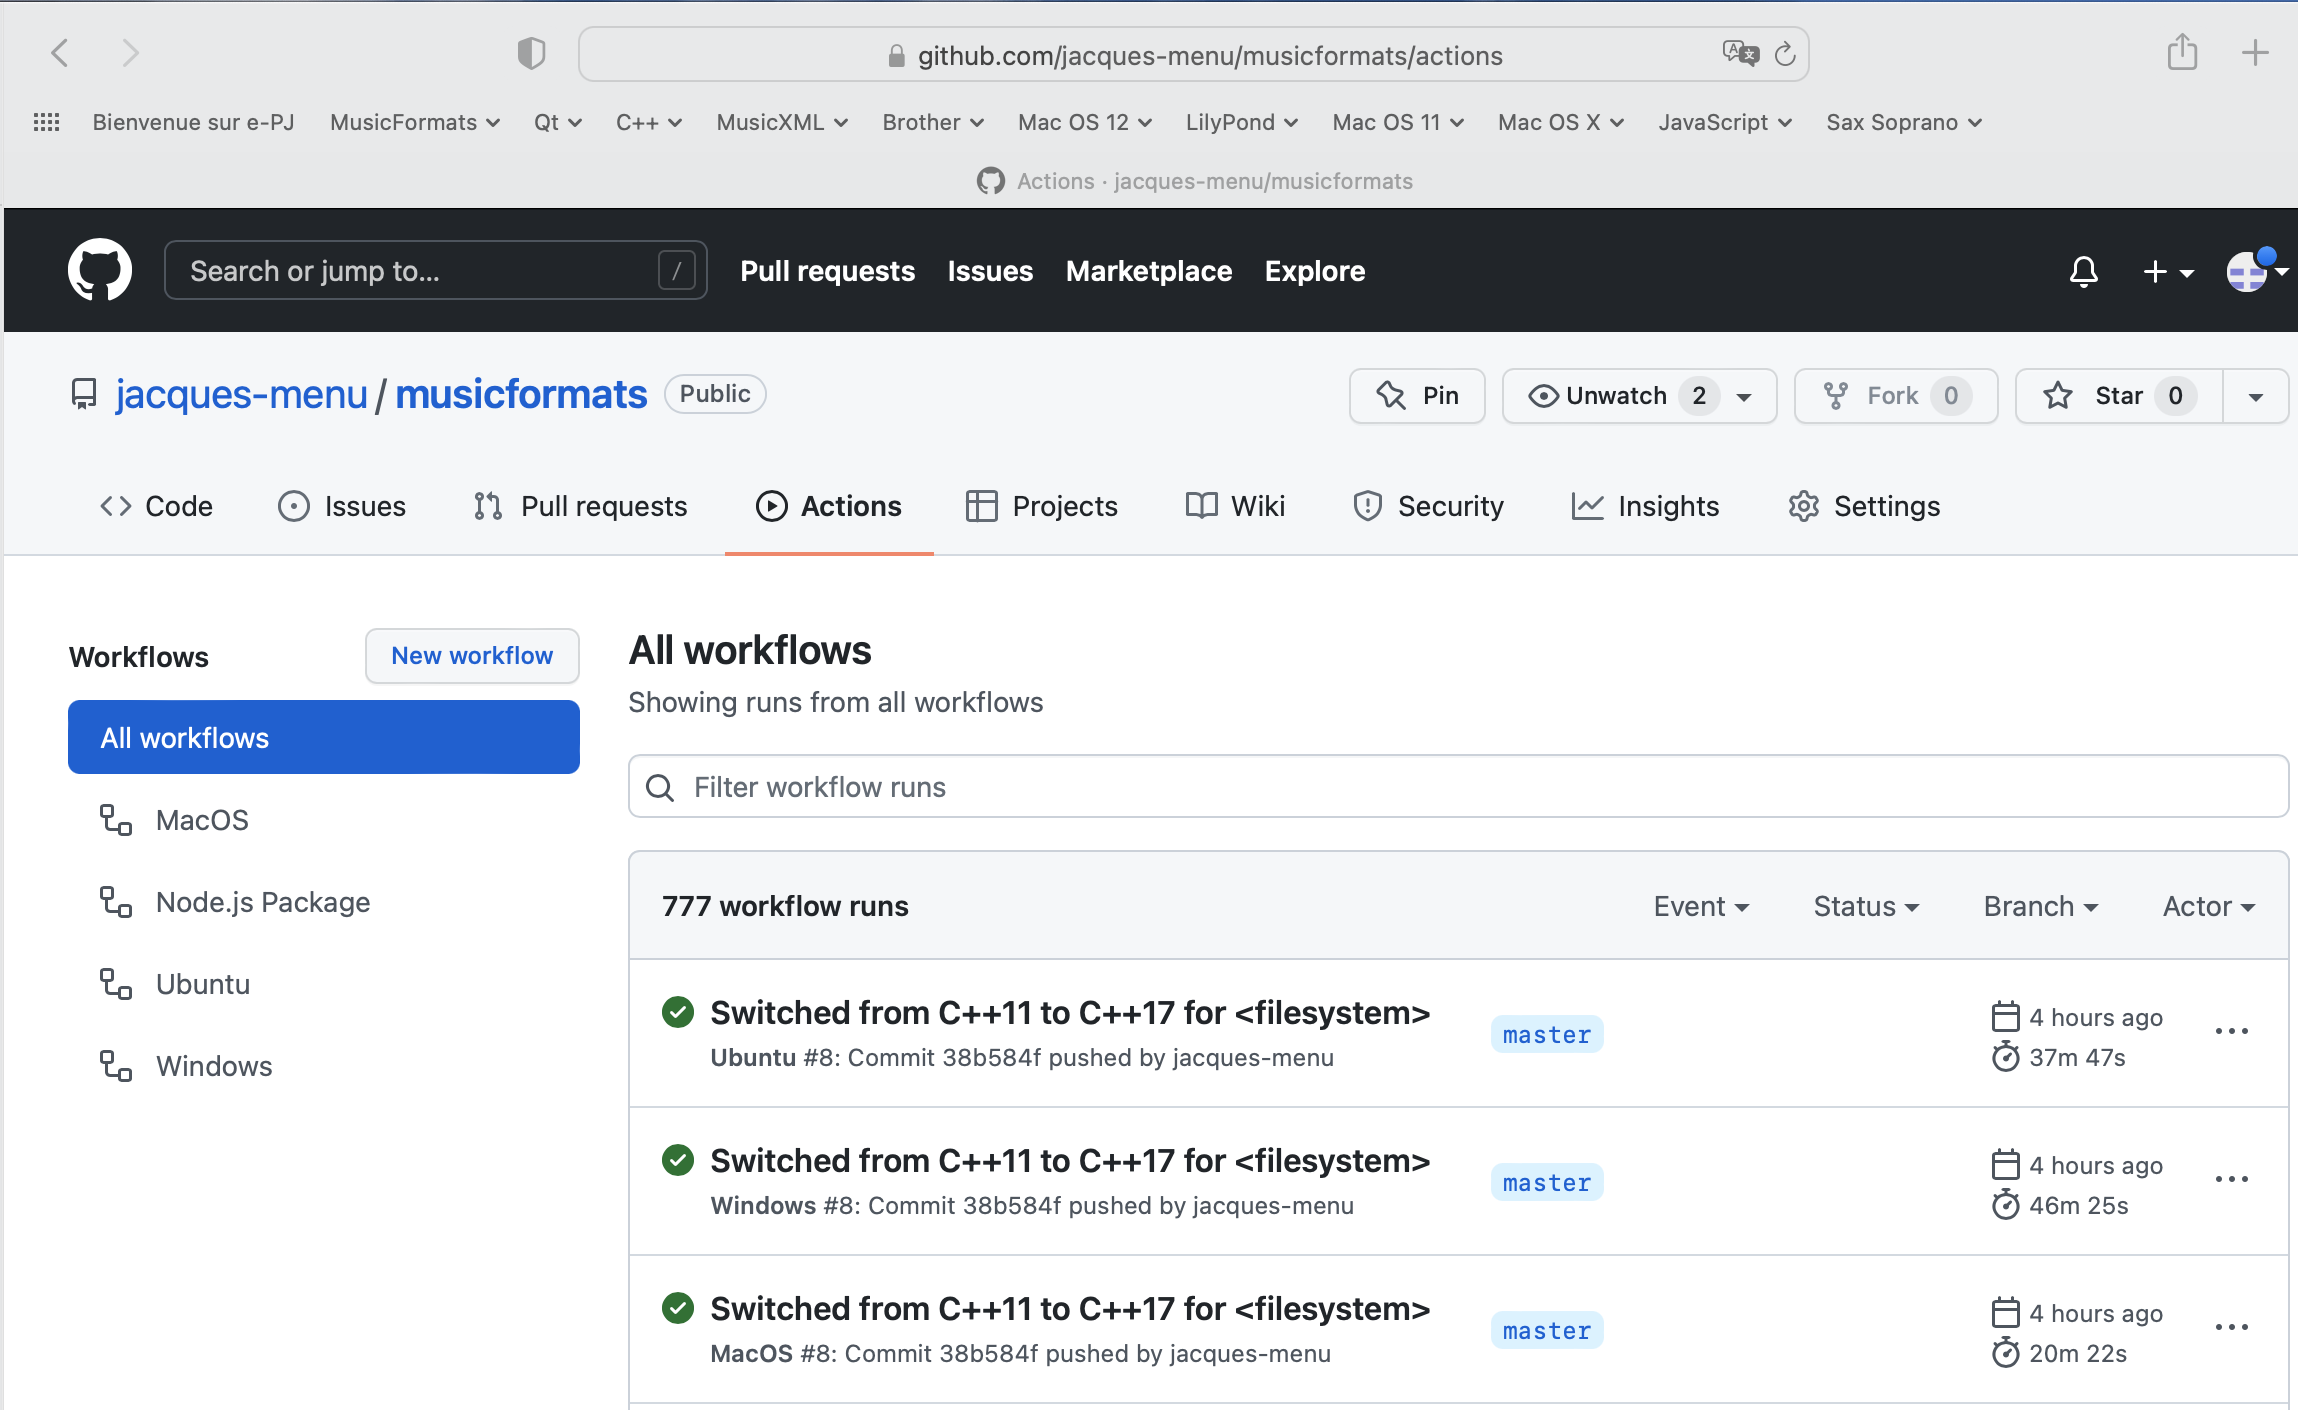
\includegraphics[scale=0.45]{../graphics/GitHubWorkflowsResults.png}

Then cliking on the link leads to:\\
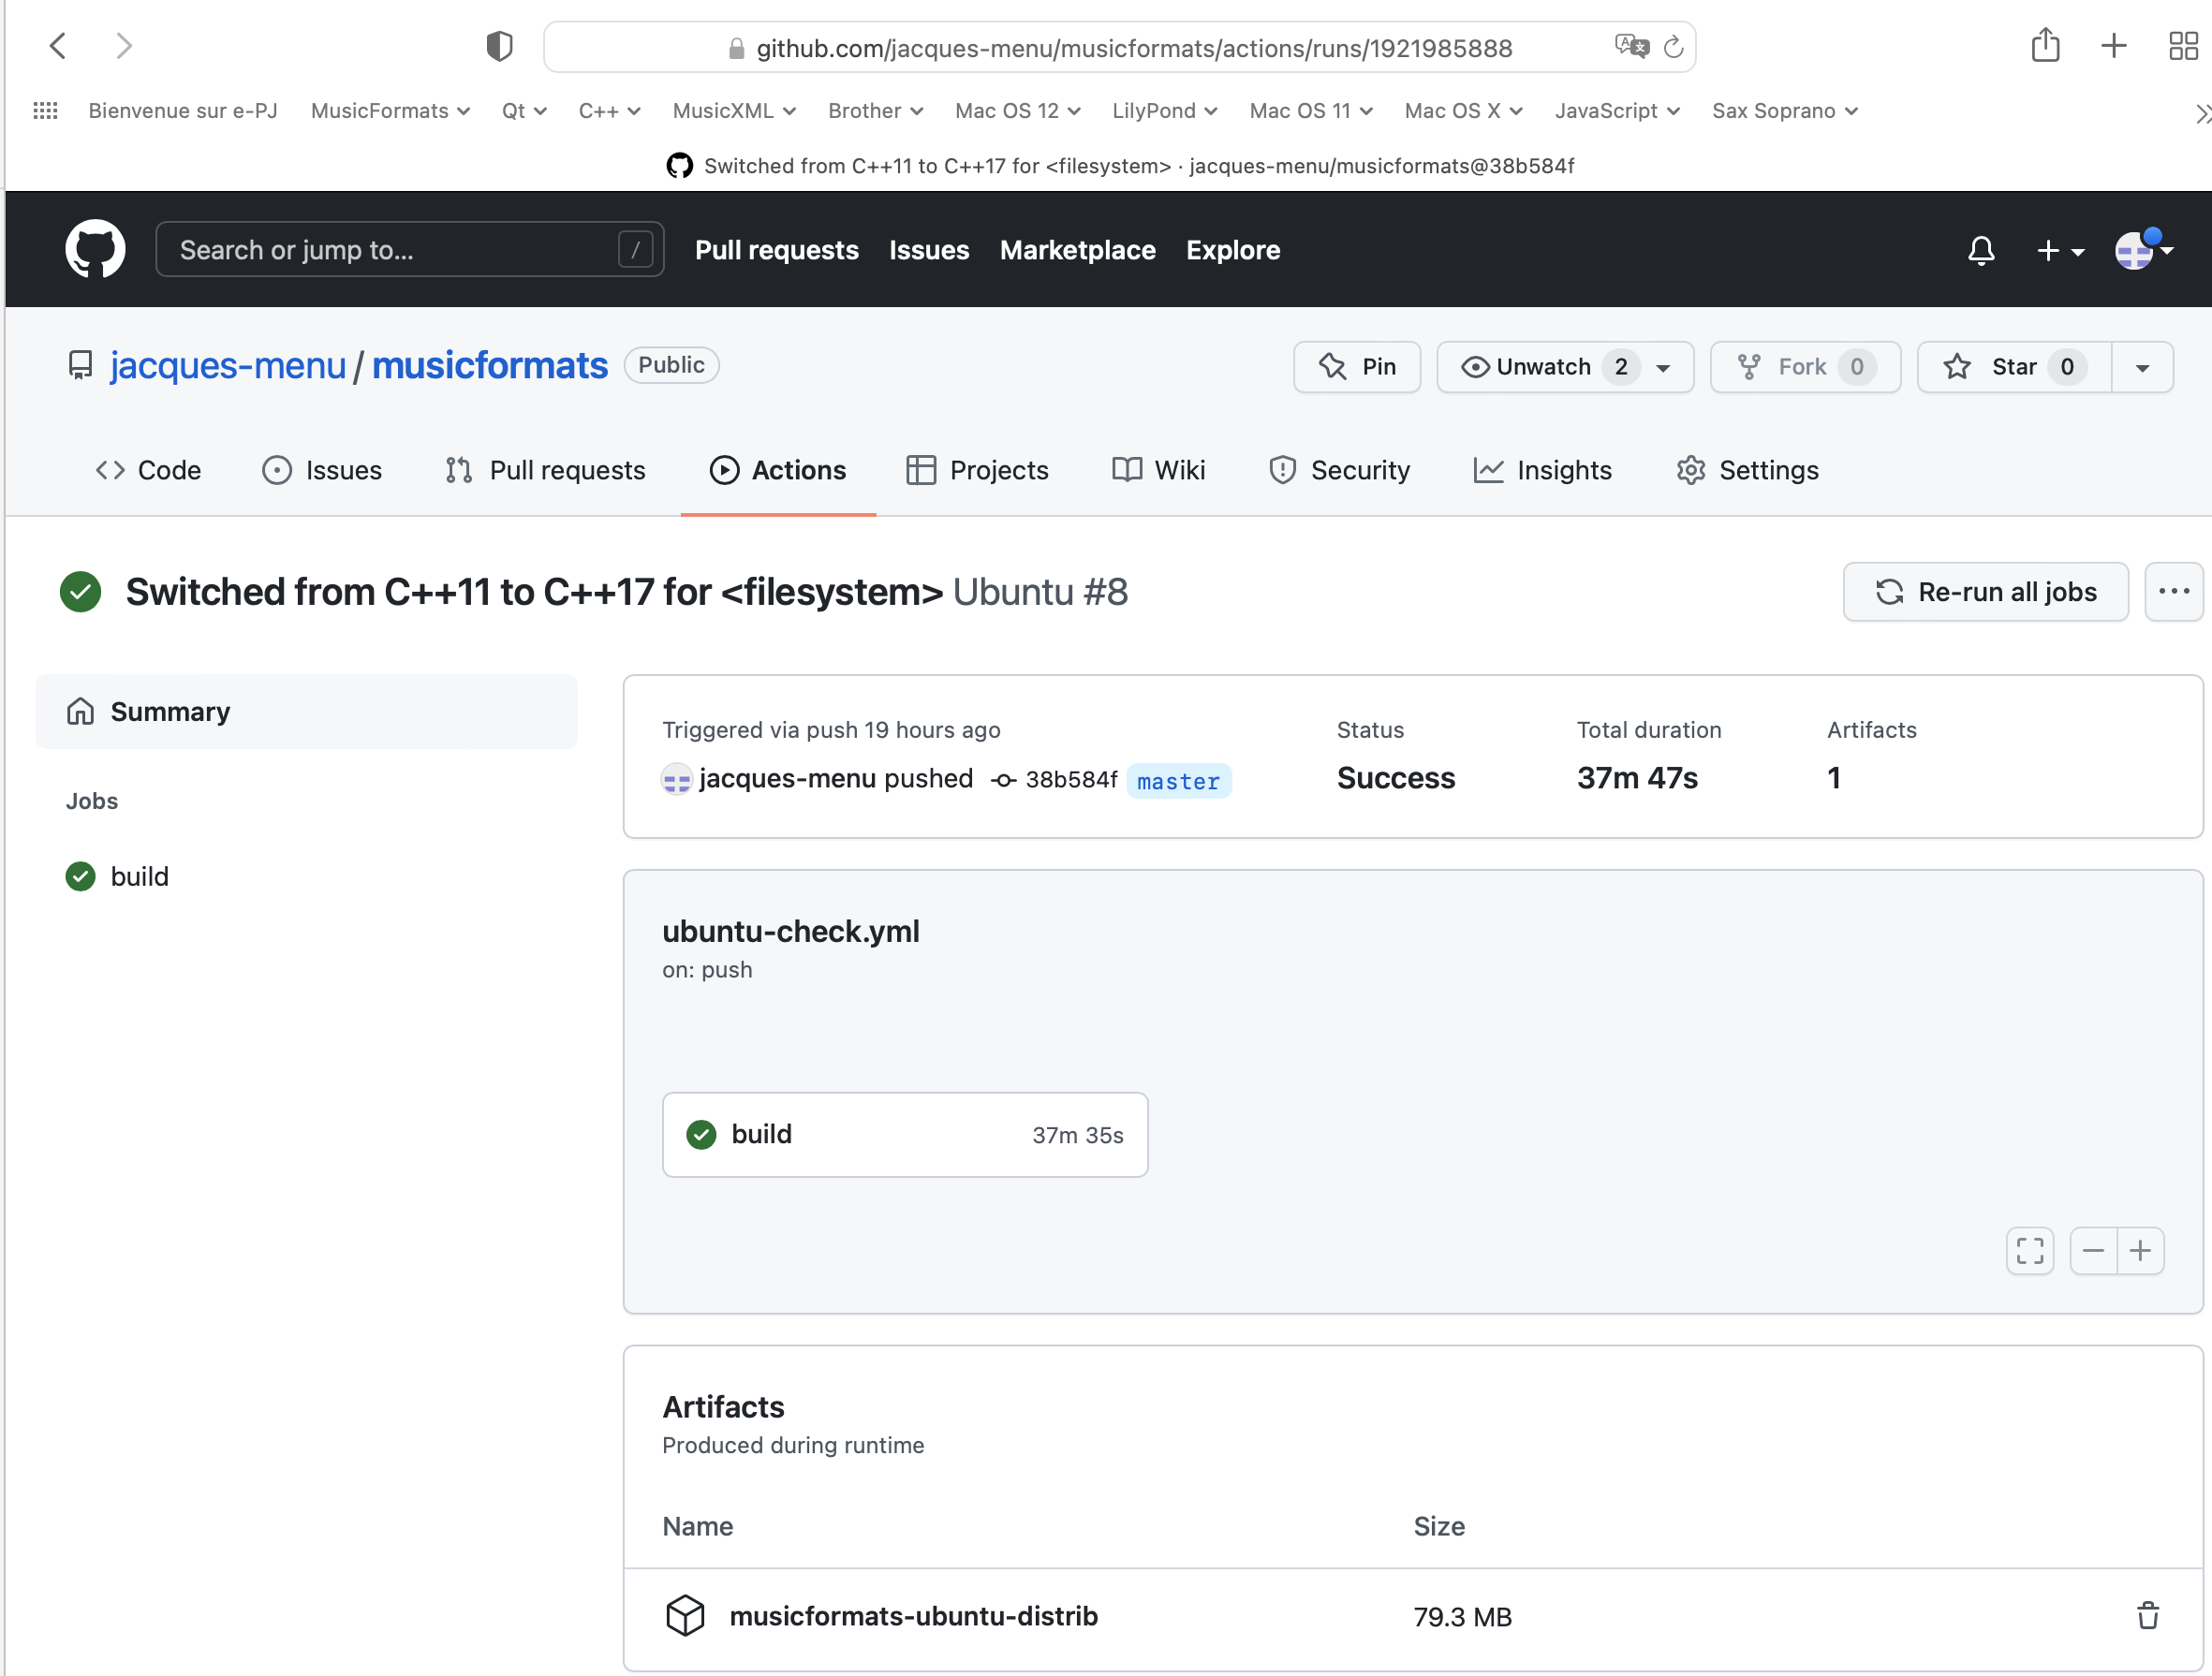
\includegraphics[scale=0.45]{../graphics/GitHubUbuntuActionResult.png}

The \code{musicformats-ubuntu-distrib} had to be clicked to get downloaded, since its URL cannot be guessed by an algorithm (it contains numbers internal to \github). Doing so for the three distributions, we get the following, here in the \directoryName{Downloads} folder on \MacOS, with the \zip\ archives implicitly uncompressed :
\begin{lstlisting}[language=Terminal]
jacquesmenu@macmini: ~/Downloads > ls -sal musicformats-*-distrib
musicformats-macos-distrib:
total 8
0 drwx------@  5 jacquesmenu  staff   160 Mar  3 07:37 .
0 drwx------+ 72 jacquesmenu  staff  2304 Mar  3 07:37 ..
8 -rw-r--r--@  1 jacquesmenu  staff     6 Mar  2 12:04 MusicFormatsVersionNumber.txt
0 drwxr-xr-x@  3 jacquesmenu  staff    96 Mar  3 07:37 build
0 drwxr-xr-x@  3 jacquesmenu  staff    96 Mar  3 07:37 documentation

musicformats-ubuntu-distrib:
total 8
0 drwx------@  5 jacquesmenu  staff   160 Mar  3 07:37 .
0 drwx------+ 72 jacquesmenu  staff  2304 Mar  3 07:37 ..
8 -rw-r--r--@  1 jacquesmenu  staff     6 Mar  2 12:22 MusicFormatsVersionNumber.txt
0 drwxr-xr-x@  4 jacquesmenu  staff   128 Mar  3 07:37 build
0 drwxr-xr-x@  3 jacquesmenu  staff    96 Mar  3 07:37 documentation

musicformats-windows-distrib:
total 8
0 drwx------@  5 jacquesmenu  staff   160 Mar  3 07:37 .
0 drwx------+ 72 jacquesmenu  staff  2304 Mar  3 07:37 ..
8 -rw-r--r--@  1 jacquesmenu  staff     6 Mar  2 12:30 MusicFormatsVersionNumber.txt
0 drwxr-xr-x@  4 jacquesmenu  staff   128 Mar  3 07:37 build
0 drwxr-xr-x@  3 jacquesmenu  staff    96 Mar  3 07:37 documentation
\end{lstlisting}


%These distributions are in the form of \zip\ files. They are are available from \url{https://github.com/jacques-menu/musicformats/tree/master/distrib}, as well as the documentation PDF files and version number:
%\begin{lstlisting}[language=Terminal]
%jacquesmenu@macmini: ~/musicformats_local_clone/distrib > ls -sal
%total 150088
%     0 drwxr-xr-x   8 jacquesmenu  staff       256 Feb 16 07:47 .
%     0 drwxr-xr-x  22 jacquesmenu  staff       704 Feb 16 07:47 ..
%  1672 -rw-r--r--   1 jacquesmenu  staff    854294 Feb 16 07:47 IntroductionToMusicXML.pdf
%  1976 -rw-r--r--   1 jacquesmenu  staff   1008702 Feb 16 07:47 MusicFormatsUserGuide.pdf
%108168 -rw-r--r--   1 jacquesmenu  staff  55378423 Feb 16 07:47 MusicFormatsForMacOS.zip
% 34080 -rw-r--r--   1 jacquesmenu  staff  17445663 Feb 16 07:47 MusicFormatsForUbuntu.zip
%  4184 -rw-r--r--   1 jacquesmenu  staff   2139537 Feb 16 07:47 MusicFormatsForWindows.zip
%     8 -rw-r--r--   1 jacquesmenu  staff         6 Feb 16 07:47 MusicFormatsVersionNumber.txt
%\end{lstlisting}

The distributions \zip\ archives are supplied with all versions, i.e. the current, most recent version of \mf (the default branch in the \repo), and the earlier versions such as the \code{v0.9.60} branch.


% -------------------------------------------------------------------------
\section{MacOS\texttrademark\ distribution}
% -------------------------------------------------------------------------

\MacOS\ software is usually distributed as \Main{DMG} files. Due to file size limitations on \github, the \MacOS\ distribution has to be compacted. This is done with \zip, and placing that in a DMG archive would not add any value. Only the \zip\ archive is thus provided.

%%%JMI\mf\ is  installable directly from the repository, since this is the environment is is developed on. Just clone the \repo\ and you will find the executables in \build{bin} and the libraries in \build{lib}.

After downloading and uncompressing \fileName{MusicFormatsForMacOS.zip}, we get:
\begin{lstlisting}[language=Terminal]
jacquesmenu@macmini: ~/Downloads/MusicFormatsForMacOS > ls -sal *
8 -rw-r--r--@ 1 jacquesmenu  staff  6 Feb 14 14:20 MusicFormatsVersionNumber.txt

bin:
total 661992
    0 drwxr-xr-x@ 25 jacquesmenu  staff       800 Feb 14 14:20 .
    0 drwxr-xr-x@  4 jacquesmenu  staff       128 Feb 15 17:23 ..
74864 -rwxr-xr-x@  1 jacquesmenu  staff  38326752 Feb 14 14:20 LilyPondIssue34
74864 -rwxr-xr-x@  1 jacquesmenu  staff  38329824 Feb 14 14:20 Mikrokosmos3Wandering
 8432 -rwxr-xr-x@  1 jacquesmenu  staff   4314896 Feb 14 14:20 MusicAndHarmonies
 8432 -rwxr-xr-x@  1 jacquesmenu  staff   4314880 Feb 14 14:20 RandomChords
 8432 -rwxr-xr-x@  1 jacquesmenu  staff   4314880 Feb 14 14:20 RandomMusic
 8624 -rwxr-xr-x@  1 jacquesmenu  staff   4414944 Feb 14 14:20 countnotes
16528 -rwxr-xr-x@  1 jacquesmenu  staff   8459424 Feb 14 14:20 displayMusicformatsHistory
16528 -rwxr-xr-x@  1 jacquesmenu  staff   8459424 Feb 14 14:20 displayMusicformatsVersion
79200 -rwxr-xr-x@  1 jacquesmenu  staff  40546384 Feb 14 14:20 msdlconverter
12480 -rwxr-xr-x@  1 jacquesmenu  staff   6387232 Feb 14 14:20 partsummary
 8848 -rwxr-xr-x@  1 jacquesmenu  staff   4528736 Feb 14 14:20 readunrolled
64000 -rwxr-xr-x@  1 jacquesmenu  staff  32764496 Feb 14 14:20 xml2brl
66872 -rwxr-xr-x@  1 jacquesmenu  staff  34236240 Feb 14 14:20 xml2gmn
17160 -rwxr-xr-x@  1 jacquesmenu  staff   8781984 Feb 14 14:20 xml2guido
67552 -rwxr-xr-x@  1 jacquesmenu  staff  34583840 Feb 14 14:20 xml2ly
12392 -rwxr-xr-x@  1 jacquesmenu  staff   6342528 Feb 14 14:20 xml2midi
59720 -rwxr-xr-x@  1 jacquesmenu  staff  30574528 Feb 14 14:20 xml2xml
 9104 -rwxr-xr-x@  1 jacquesmenu  staff   4657200 Feb 14 14:20 xmlclone
 9256 -rwxr-xr-x@  1 jacquesmenu  staff   4735296 Feb 14 14:20 xmlfactory
 8800 -rwxr-xr-x@  1 jacquesmenu  staff   4504976 Feb 14 14:20 xmliter
 8680 -rwxr-xr-x@  1 jacquesmenu  staff   4442496 Feb 14 14:20 xmlread
11976 -rwxr-xr-x@  1 jacquesmenu  staff   6129744 Feb 14 14:20 xmltranspose
 9248 -rwxr-xr-x@  1 jacquesmenu  staff   4734368 Feb 14 14:20 xmlversion
\end{lstlisting}

\MacOS\ executables are self-sufficient and can be placed anywhere on a disk except the trash. Usually, there are placed in the \code{/Applications} directory.


% -------------------------------------------------------------------------
\subsection{Security issue in recent MacOS\texttrademark\ versions}
% -------------------------------------------------------------------------

\MacOS\ gets more and more stringent over time regarding security. The \OS\ part in charge of this is named \Gatekeeper.

When installing \mf\ from the \repo\ on versions up to 10 (\Main{High Sierra}), the executables in \code{bin} are usable alright.

From version 11 (\Main{Catalina}) on, though, the executables you get are not executable actually, because their developer is unknown to the \OS, and actions have to be taken for them to be usable.

The screenshot below has been made with \MacOS\ \Main{Monterey} 12.0.1 with english as the user interface language. The texts vary of course depending on the language used.

When launching one of these executables for the first time, such as:
\begin{lstlisting}[language=Terminal]
jacquesmenu@macmini: ~/Downloads/MusicFormatsForMacOS/bin > ./xml2ly
\end{lstlisting}
we get a alert telling that it cannot be opened, because the developper is not known to the \OS:\\
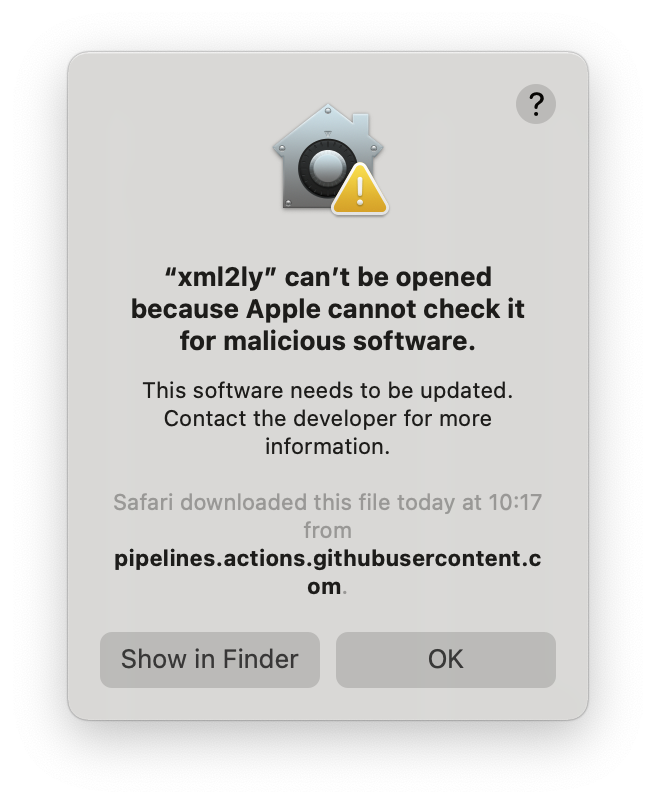
\includegraphics[scale=0.35]{../graphics/MacOSMaliciousSoftwareAlert.png}

Clicking in either buttons in this dialog kill the process:
\begin{lstlisting}[language=Terminal]
Killed: 9
\end{lstlisting}

The trouble is that these executables are in {\it \quarantine} by default. To make them usable, they have to quit quarantine, which is done by removing one of their attributes:
\begin{lstlisting}[language=Terminal]
jacquesmenu@macmini: ~/Downloads/MusicFormatsForMacOS/bin > xattr -d com.apple.quarantine *
\end{lstlisting}
%codesign --sign - --force --deep %%%JMI not necessary

From then on, the \mf\ executables can be used seamlessly on the given machine.

Having to perform the preceding task for each executable is the price to pay for security. And it has to be perfomed again when installing new versions\dots


The above can be done in the \GUI\ file by file too. Right after you got the message above:
\begin{itemize}
\item  open \MainIt{System Preferences}, choose the \MainIt{Security \& Privacy} tab, and there click on the \MainIt{General button};

\item click on the lock at the bottom left of the dialog to make changes:\\
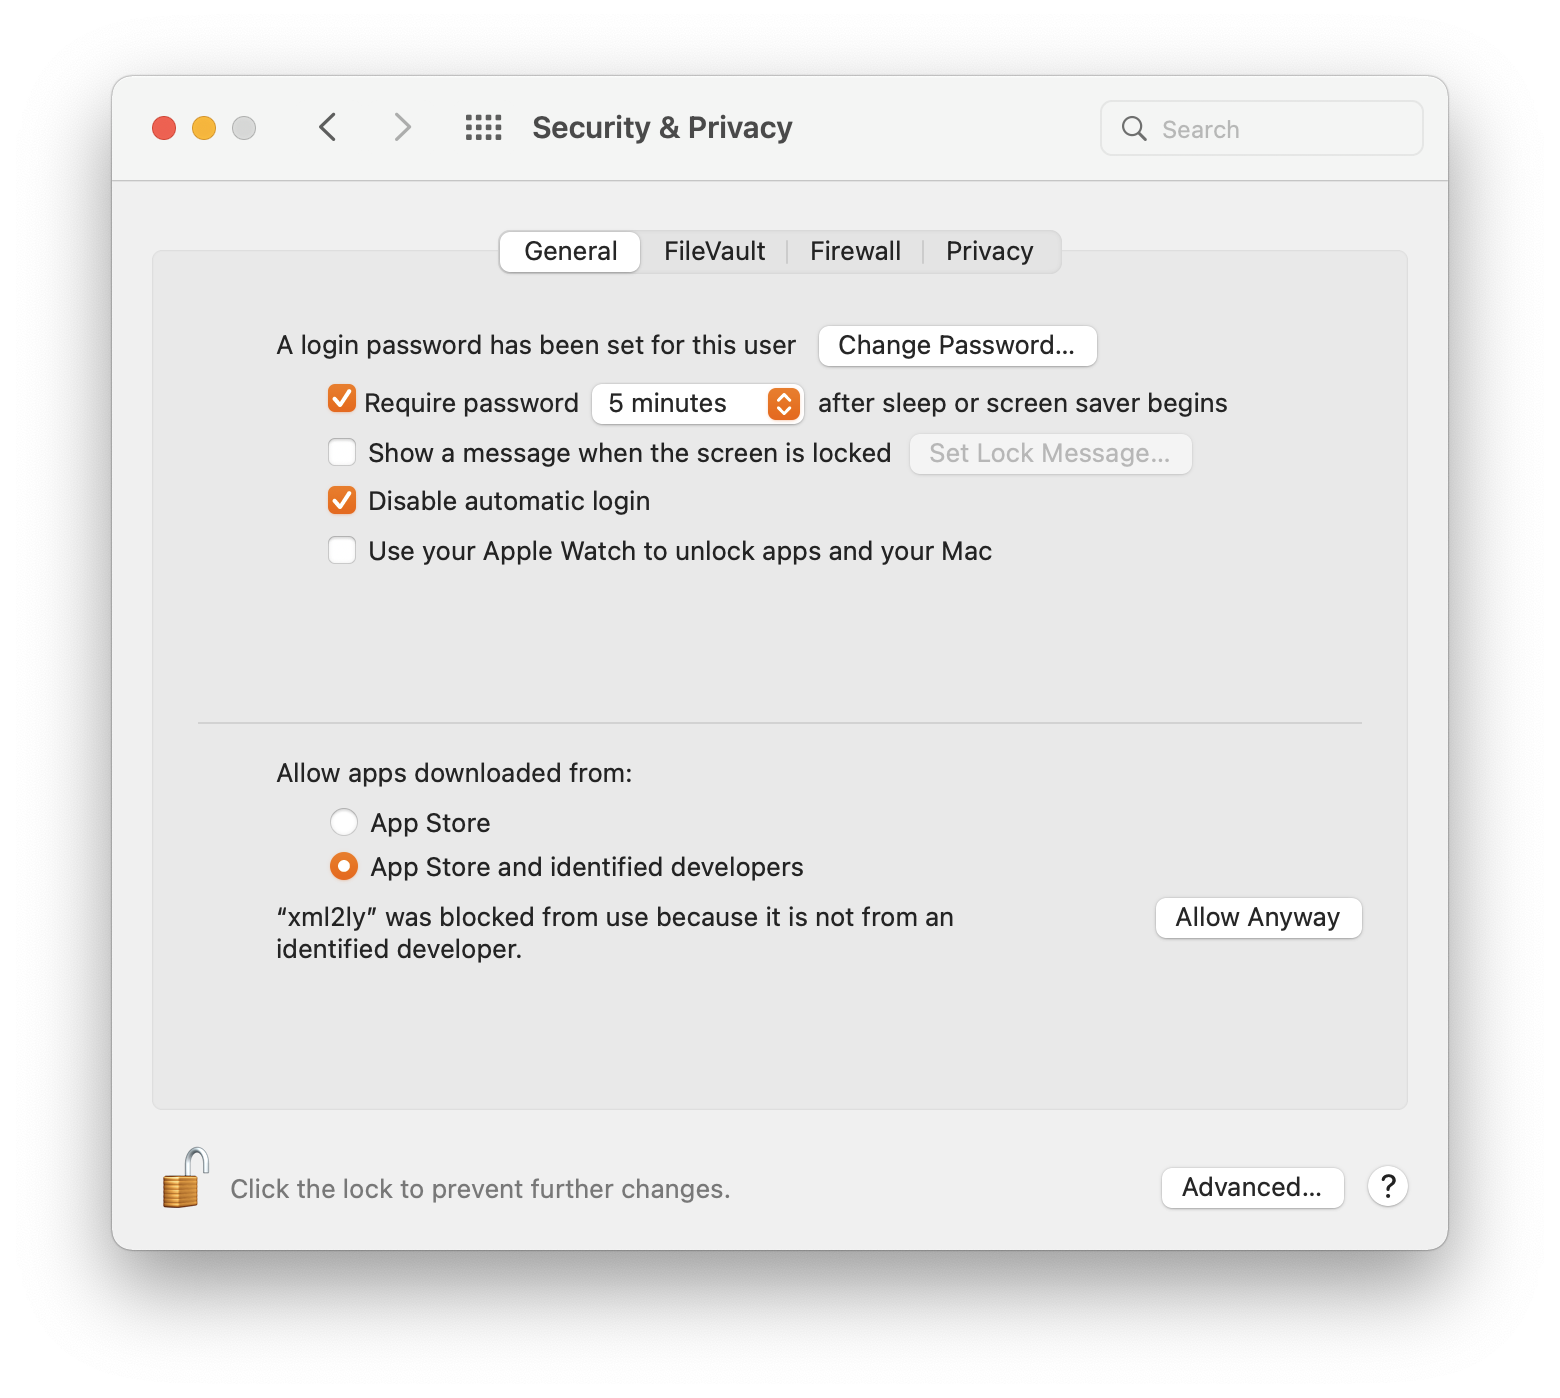
\includegraphics[scale=0.35]{../graphics/MacOSAllowAnyway.png}

\item click on the \MainIt{Allow Anyway} button.
%%%JMI sudo spctl --master-disable to create a Anywhere radio button
%jacquesmenu@macmini > spctl --status
%assessments enabled

\end{itemize}

Re-execute the executable from the command line. This pops-up a dialog to confirm you actually want to use this software:\\
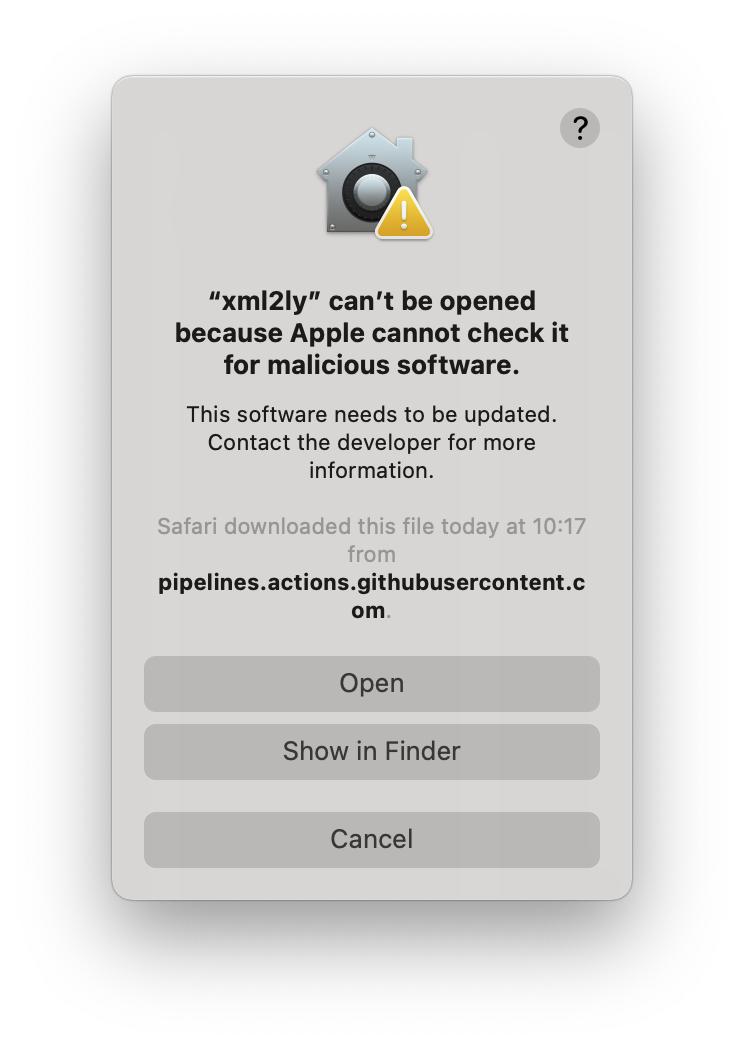
\includegraphics[scale=0.35]{../graphics/MacOSConfirmOpening.png}

Click on the \MainIt{Open} button to register the executable in \Gatekeeper\ and go ahead.


% -------------------------------------------------------------------------
\section{Ubuntu distribution}
% -------------------------------------------------------------------------

After downloading, we get:
\begin{lstlisting}[language=Terminal]
jacquesmenu@macmini: ~/Downloads/MusicFormatsForUbuntu > ls -sal *
8 -rw-r--r--@ 1 jacquesmenu  staff  6 Feb 14 14:33 MusicFormatsVersionNumber.txt

bin:
total 2296
  0 drwxr-xr-x@ 25 jacquesmenu  staff     800 Feb 14 18:22 .
  0 drwxr-xr-x@  6 jacquesmenu  staff     192 Feb 16 08:45 ..
 96 -rw-r--r--@  1 jacquesmenu  staff   49000 Feb 14 14:33 LilyPondIssue34
 96 -rw-r--r--@  1 jacquesmenu  staff   49040 Feb 14 14:33 Mikrokosmos3Wandering
 96 -rw-r--r--@  1 jacquesmenu  staff   47224 Feb 14 14:33 MusicAndHarmonies
 96 -rw-r--r--@  1 jacquesmenu  staff   47216 Feb 14 14:33 RandomChords
 96 -rw-r--r--@  1 jacquesmenu  staff   47216 Feb 14 14:33 RandomMusic
 72 -rw-r--r--@  1 jacquesmenu  staff   33800 Feb 14 14:33 countnotes
 40 -rw-r--r--@  1 jacquesmenu  staff   17648 Feb 14 14:33 displayMusicformatsHistory
 40 -rw-r--r--@  1 jacquesmenu  staff   17648 Feb 14 14:33 displayMusicformatsVersion
104 -rw-r--r--@  1 jacquesmenu  staff   50616 Feb 14 14:33 msdlconverter
544 -rw-r--r--@  1 jacquesmenu  staff  275976 Feb 14 14:33 partsummary
 88 -rw-r--r--@  1 jacquesmenu  staff   43720 Feb 14 14:33 readunrolled
 80 -rw-r--r--@  1 jacquesmenu  staff   39200 Feb 14 14:33 xml2brl
 88 -rw-r--r--@  1 jacquesmenu  staff   43336 Feb 14 14:33 xml2gmn
 48 -rw-r--r--@  1 jacquesmenu  staff   23112 Feb 14 14:33 xml2guido
 80 -rw-r--r--@  1 jacquesmenu  staff   39056 Feb 14 14:33 xml2ly
 88 -rw-r--r--@  1 jacquesmenu  staff   42880 Feb 14 14:33 xml2midi
 88 -rw-r--r--@  1 jacquesmenu  staff   43344 Feb 14 14:33 xml2xml
 88 -rw-r--r--@  1 jacquesmenu  staff   43368 Feb 14 14:33 xmlclone
 48 -rw-r--r--@  1 jacquesmenu  staff   22616 Feb 14 14:33 xmlfactory
168 -rw-r--r--@  1 jacquesmenu  staff   83488 Feb 14 14:33 xmliter
 56 -rw-r--r--@  1 jacquesmenu  staff   28424 Feb 14 14:33 xmlread
 56 -rw-r--r--@  1 jacquesmenu  staff   28656 Feb 14 14:33 xmltranspose
 40 -rw-r--r--@  1 jacquesmenu  staff   17360 Feb 14 14:33 xmlversion

lib:
total 157792
     0 drwxr-xr-x@ 4 jacquesmenu  staff       128 Feb 14 18:22 .
     0 drwxr-xr-x@ 6 jacquesmenu  staff       192 Feb 16 08:45 ..
113224 -rw-r--r--@ 1 jacquesmenu  staff  57968176 Feb 14 14:33 libmusicxml2.a
 44568 -rw-r--r--@ 1 jacquesmenu  staff  22818696 Feb 14 14:33 libmusicxml2.so
\end{lstlisting}

Move the \fileName{MusicFormatsForUbuntu} directory to a suitable place and set your \code{PATH} and \code{LIBRARY_PATH} \environmentVariable s accordingly.


% -------------------------------------------------------------------------
\section{Windows\texttrademark\ distribution}
% -------------------------------------------------------------------------

After downloading, we get:
\begin{lstlisting}[language=Terminal]
jacquesmenu@macmini: ~/Downloads/MusicFormatsForWindows > ls -sal *
8 -rw-r--r--@ 1 jacquesmenu  staff  6 Feb 14 14:53 MusicFormatsVersionNumber.txt

bin:
total 1232
  0 drwxr-xr-x@ 25 jacquesmenu  staff    800 Feb 14 18:22 .
  0 drwxr-xr-x@  6 jacquesmenu  staff    192 Feb 16 08:49 ..
 80 -rw-r--r--@  1 jacquesmenu  staff  38400 Feb 14 14:53 LilyPondIssue34.exe
 80 -rw-r--r--@  1 jacquesmenu  staff  38400 Feb 14 14:53 Mikrokosmos3Wandering.exe
 56 -rw-r--r--@  1 jacquesmenu  staff  26112 Feb 14 14:53 MusicAndHarmonies.exe
 56 -rw-r--r--@  1 jacquesmenu  staff  25088 Feb 14 14:53 RandomChords.exe
 56 -rw-r--r--@  1 jacquesmenu  staff  25088 Feb 14 14:53 RandomMusic.exe
 32 -rw-r--r--@  1 jacquesmenu  staff  14848 Feb 14 14:53 countnotes.exe
 24 -rw-r--r--@  1 jacquesmenu  staff  10752 Feb 14 14:53 displayMusicformatsHistory.exe
 24 -rw-r--r--@  1 jacquesmenu  staff  10752 Feb 14 14:53 displayMusicformatsVersion.exe
 80 -rw-r--r--@  1 jacquesmenu  staff  39936 Feb 14 14:53 msdlconverter.exe
112 -rw-r--r--@  1 jacquesmenu  staff  56832 Feb 14 14:53 partsummary.exe
 40 -rw-r--r--@  1 jacquesmenu  staff  18432 Feb 14 14:53 readunrolled.exe
 64 -rw-r--r--@  1 jacquesmenu  staff  32768 Feb 14 14:53 xml2brl.exe
 72 -rw-r--r--@  1 jacquesmenu  staff  33280 Feb 14 14:53 xml2gmn.exe
 64 -rw-r--r--@  1 jacquesmenu  staff  29184 Feb 14 14:53 xml2guido.exe
 64 -rw-r--r--@  1 jacquesmenu  staff  32768 Feb 14 14:53 xml2ly.exe
 40 -rw-r--r--@  1 jacquesmenu  staff  17920 Feb 14 14:53 xml2midi.exe
 72 -rw-r--r--@  1 jacquesmenu  staff  33280 Feb 14 14:53 xml2xml.exe
 32 -rw-r--r--@  1 jacquesmenu  staff  14848 Feb 14 14:53 xmlclone.exe
 32 -rw-r--r--@  1 jacquesmenu  staff  15360 Feb 14 14:53 xmlfactory.exe
 40 -rw-r--r--@  1 jacquesmenu  staff  19456 Feb 14 14:53 xmliter.exe
 56 -rw-r--r--@  1 jacquesmenu  staff  27136 Feb 14 14:53 xmlread.exe
 32 -rw-r--r--@  1 jacquesmenu  staff  14848 Feb 14 14:53 xmltranspose.exe
 24 -rw-r--r--@  1 jacquesmenu  staff  12288 Feb 14 14:53 xmlversion.exe

lib:
total 37368
    0 drwxr-xr-x@ 4 jacquesmenu  staff       128 Feb 14 18:22 .
    0 drwxr-xr-x@ 6 jacquesmenu  staff       192 Feb 16 08:49 ..
14696 -rw-r--r--@ 1 jacquesmenu  staff   7521356 Feb 14 14:53 musicxml2.exp
22672 -rw-r--r--@ 1 jacquesmenu  staff  11604836 Feb 14 14:53 musicxml2.lib
\end{lstlisting}

Move the \fileName{MusicFormatsForUbuntu} directory to a suitable place such as \code{C:\textbackslash\ Program Files} and set your \code{PATH} \environmentVariable\ accordingly.


